\documentclass[tikz,svgnames]{standalone}

\usetikzlibrary{mindmap}

\begin{document}

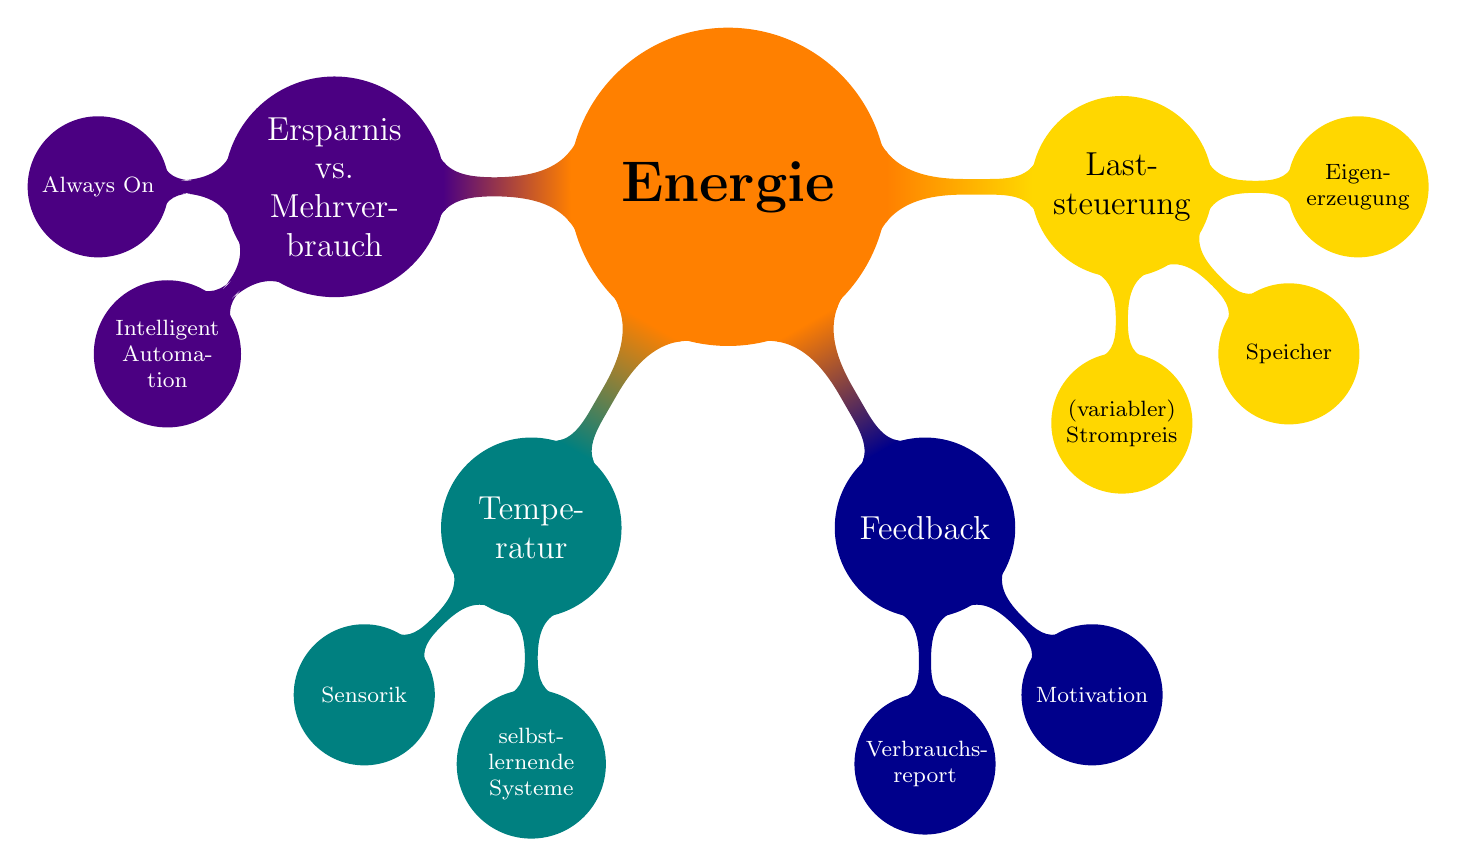
\begin{tikzpicture}[
    mindmap, grow cyclic, every node/.style=concept, concept color=orange,
    level 1/.append style={level distance=5cm,sibling angle=60,font=\large},
    level 2/.append style={level distance=3cm,sibling angle=45}
  ]

  \node{\textbf{\huge{Energie}}} [clockwise from=0]
  child [concept color=Gold] { node {Last\-steuerung} [clockwise from=0]
      child { node {Eigen\-erzeugung}}
      child { node {Speicher}}
      child { node {(variabler) Strompreis}}
    }
  child [concept color=DarkBlue,text=white] { node {Feedback} [counterclockwise from=270]
      child { node {Verbrauchs\-report}}
      child { node {Motivation}}
    }
  child [concept color=teal,text=white] { node {Tempe\-ratur} [clockwise from=270]
      child { node {selbst\-lernende Systeme}}
      child { node {Sensorik}}
    }
  child [concept color=Indigo,text=white] { node {Ersparnis vs. Mehrverbrauch} [counterclockwise from=180]
      child { node {Always On}}
      child { node {Intelligent Automation}}
    };
\end{tikzpicture}

\end{document}
